\documentclass[conference]{IEEEtran}
\IEEEoverridecommandlockouts
% The preceding line is only needed to identify funding in the first footnote. If that is unneeded, please comment it out.
\usepackage{cite}
\usepackage{amsmath,amssymb,amsfonts}
\usepackage{algorithmic}
\usepackage{graphicx}
\usepackage{textcomp}
\usepackage{xcolor}

\newcommand{\todo}[1]{\textbf{\textcolor{red}{To do: #1}}}
\newcommand{\csp}[1]{\textbf{\textcolor{purple}{CSP: #1}}}
\newcommand{\ryo}[1]{\textbf{\textcolor{teal}{RY: #1}}}

\makeatletter
\newcommand{\linebreakand}{%
  \end{@IEEEauthorhalign}
  \hfill\mbox{}\par
  \mbox{}\hfill\begin{@IEEEauthorhalign}
}
\makeatother

\begin{document}

\title{OptoFlood: Controllable Flooding for NDN Producer Mobility\\
\thanks{Identify applicable funding agency here. If none, delete this.}
}

\author{
    \IEEEauthorblockN{Yuting Wan}
    \IEEEauthorblockA{University of Glasgow\\
    yuting.wan@glasgow.ac.uk}
\and
    \IEEEauthorblockN{Ryo Yanagida}
    \IEEEauthorblockA{University of Glasgow\\
    ryo@htonl.net}
\and
    \IEEEauthorblockN{Paul Harvey}
    \IEEEauthorblockA{University of Glasgow\\
    paul.harvey@glasgow.ac.uk}
\linebreakand
    \IEEEauthorblockN{Jeremy Singer}
    \IEEEauthorblockA{University of Glasgow\\
    jeremy.singer@glasgow.ac.uk}
\and
    \IEEEauthorblockN{Colin Perkins}
    \IEEEauthorblockA{University of Glasgow\\
    csp@csperkins.org}
\and
    \IEEEauthorblockN{XXX}
    \IEEEauthorblockA{Rakuten Mobile\\
    xxx@rakuten.com}
}

\maketitle

\begin{abstract}

Producer mobility in Named Data Networking (NDN) results in increased latency and packet loss due to slow global routing convergence. This affects latency-sensitive applications, such as live video streaming and video conferencing, where even brief interruptions degrade user experience. To address this, we propose \textit{OptoFlood}, a controllable flooding mechanism that proactively manages both Data and Interest packets immediately following producer movements, rapidly establishing temporary bidirectional communication paths. OptoFlood also accelerates global routing convergence through integration with the Named-data Link State Routing (NLSR) protocol. Our initial evaluation demonstrates that OptoFlood effectively reduces latency and packet loss, caused by producer mobility, while maintaining low network overhead.

\end{abstract}

\begin{IEEEkeywords}
Named Data Networking, Producer Mobility, NLSR, Routing
\end{IEEEkeywords}


\section{Introduction} \label{sec:introduction}

% Paragraph 1: Motivation.
Named Data Networking (NDN) provides data-centric communication, improving network efficiency primarily through named data retrieval and in-network caching mechanisms. However, producer mobility remains a significant challenge in dynamic network environments. Each time a producer moves, the network must quickly discover its new location and ensure continuous data delivery without introducing delays or packet loss. In scenarios such as live video streaming on smartphones or mobile video conferencing while switching between WiFi hotspots, even short interruptions can severely degrade the user experience and reliability. Addressing producer mobility is therefore essential to ensuring the stability and responsiveness of NDN, particularly for latency-sensitive applications.

% Paragraph 2: Specific problem.
We consider the delay and packet loss caused by the slow routing convergence when NDN producers change their network attachment point. NDN producers must re-register their data prefix at each new network location and wait for global routing updates to propagate. During this convergence period, Interest packets may be misrouted or discarded due to outdated forwarding paths. Our baseline tests indicate that this can result in interruptions lasting several seconds, severely impacting latency-sensitive applications. In addition, repeated movements can exacerbate this issue, significantly affecting the overall performance of the network.

% Paragraph 3: Contributions.
In this paper, we propose OptoFlood, a controllable flooding mechanism designed to rapidly establish temporary bidirectional communication paths and accelerate network convergence immediately after producer mobility events. OptoFlood proactively manages flooding of both Data and Interest packets, enabling rapid recovery from disruptions caused by producer movements. Producers initiate flooding by transmitting specially marked Data packets corresponding specifically to pending Interests received before the movement. These flooded packets are constrained to reach nodes that remain on, or near, the original forwarding path, thus rescuing Interests without waiting for global routing updates. Meanwhile, intermediate forwarders detecting invalidated forwarding entries perform Interest flooding with strictly limited propagation scopes, such as constrained hop counts, to efficiently locate the producer’s new attachment point. Finally, OptoFlood integrates its flooding results with Named-data Link State Routing (NLSR), generating short-lived routing updates based on newly established temporary paths. This integration accelerates global routing convergence. Collectively, these mechanisms reduce latency and packet loss while maintaining low overhead in network resource usage.

% Paragraph 4: Comparison to related work.
Compared to existing NDN mobility approaches, such as routing-based updates \cite{meddeb:2018:afirm}, Interest-based notification solutions \cite{auge:2016:map-me} or anchor-based tracing mechanisms \cite{zhang:2018:kite},
OptoFlood provides a more integrated and lightweight solution that leverages flooding as its primary mechanism for instant path recovery and rapid convergence. Unlike existing flooding solutions, our approach uses explicit controls, including hop limits and producer-side flood rate limits, to restrict the scope and duration of flooding, minimising unnecessary overhead. Additionally, by leveraging temporary bidirectional paths established via controlled flooding, OptoFlood-Hybrid accelerates global routing updates locally without relying on centralised anchor nodes, thereby avoiding single points of failure and reducing potential path inefficiencies.

% Paragraph 5: Roadmap.
We structure the remainder of this paper as follows. Section \ref{sec:problem} reviews the background of producer mobility problems in NDN, highlighting the limitations of traditional routing updates. Section \ref{sec:solution} presents the detailed design of OptoFlood, including the mechanisms for controlled flooding of Data and Interest packets, and the integration with NLSR to accelerate global convergence. Section \ref{sec:evaluation} describes our experimental setup and presents results that demonstrate the effectiveness of our approach. Finally, Section \ref{sec:conclusion} concludes the paper and briefly discusses potential directions for future enhancements of the OptoFlood approach.


\section{Producer Mobility Problems in NDN}
\label{sec:problem}

\subsection{NDN Background}

Named Data Networking (NDN) shifts from traditional IP-based host-centric communication to a data-centric model, where content is identified by names rather than addresses. In NDN, communication relies on two core packet types: \textit{Interest Packets}, sent by consumers to request data by specifying the content name, and \textit{Data Packets}, returned by producers containing the requested content and related metadata. Both packet types follow a concise Type-Length-Value (TLV) encoding, enabling efficient processing and extensibility.

Each NDN forwarder maintains three essential data structures to handle packet forwarding:

\begin{itemize}
    \item \textbf{Content Store (CS):} A cache that temporarily stores passing data packets, enabling immediate response to repeated requests.
    \item \textbf{Pending Interest Table (PIT):} Records forwarded Interest packets awaiting the corresponding Data packets, ensuring accurate reverse path forwarding.
    \item \textbf{Forwarding Information Base (FIB):} Stores routing information mapping name prefixes to outgoing interfaces, guiding Interest Packet forwarding decisions.
\end{itemize}

When an Interest Packet arrives at a forwarder, the node first checks its CS for the requested content. If the data are available, it immediately returns the cached Data Packet. If not, the forwarder looks up the PIT. If an identical interest is already pending, the forwarder aggregates this new request instead of forwarding it again. Otherwise, it forwards the Interest Packet according to the matching entry in the FIB and records the interest in the PIT. Upon reaching a node (either the original producer or an intermediate cache) that possesses the desired content, a Data Packet is sent back along the reverse path traced by PIT entries. Figure~\ref{fig:NDN Packets Processing Flow} illustrates packet forwarding.

\begin{figure}[t]
    \centering
    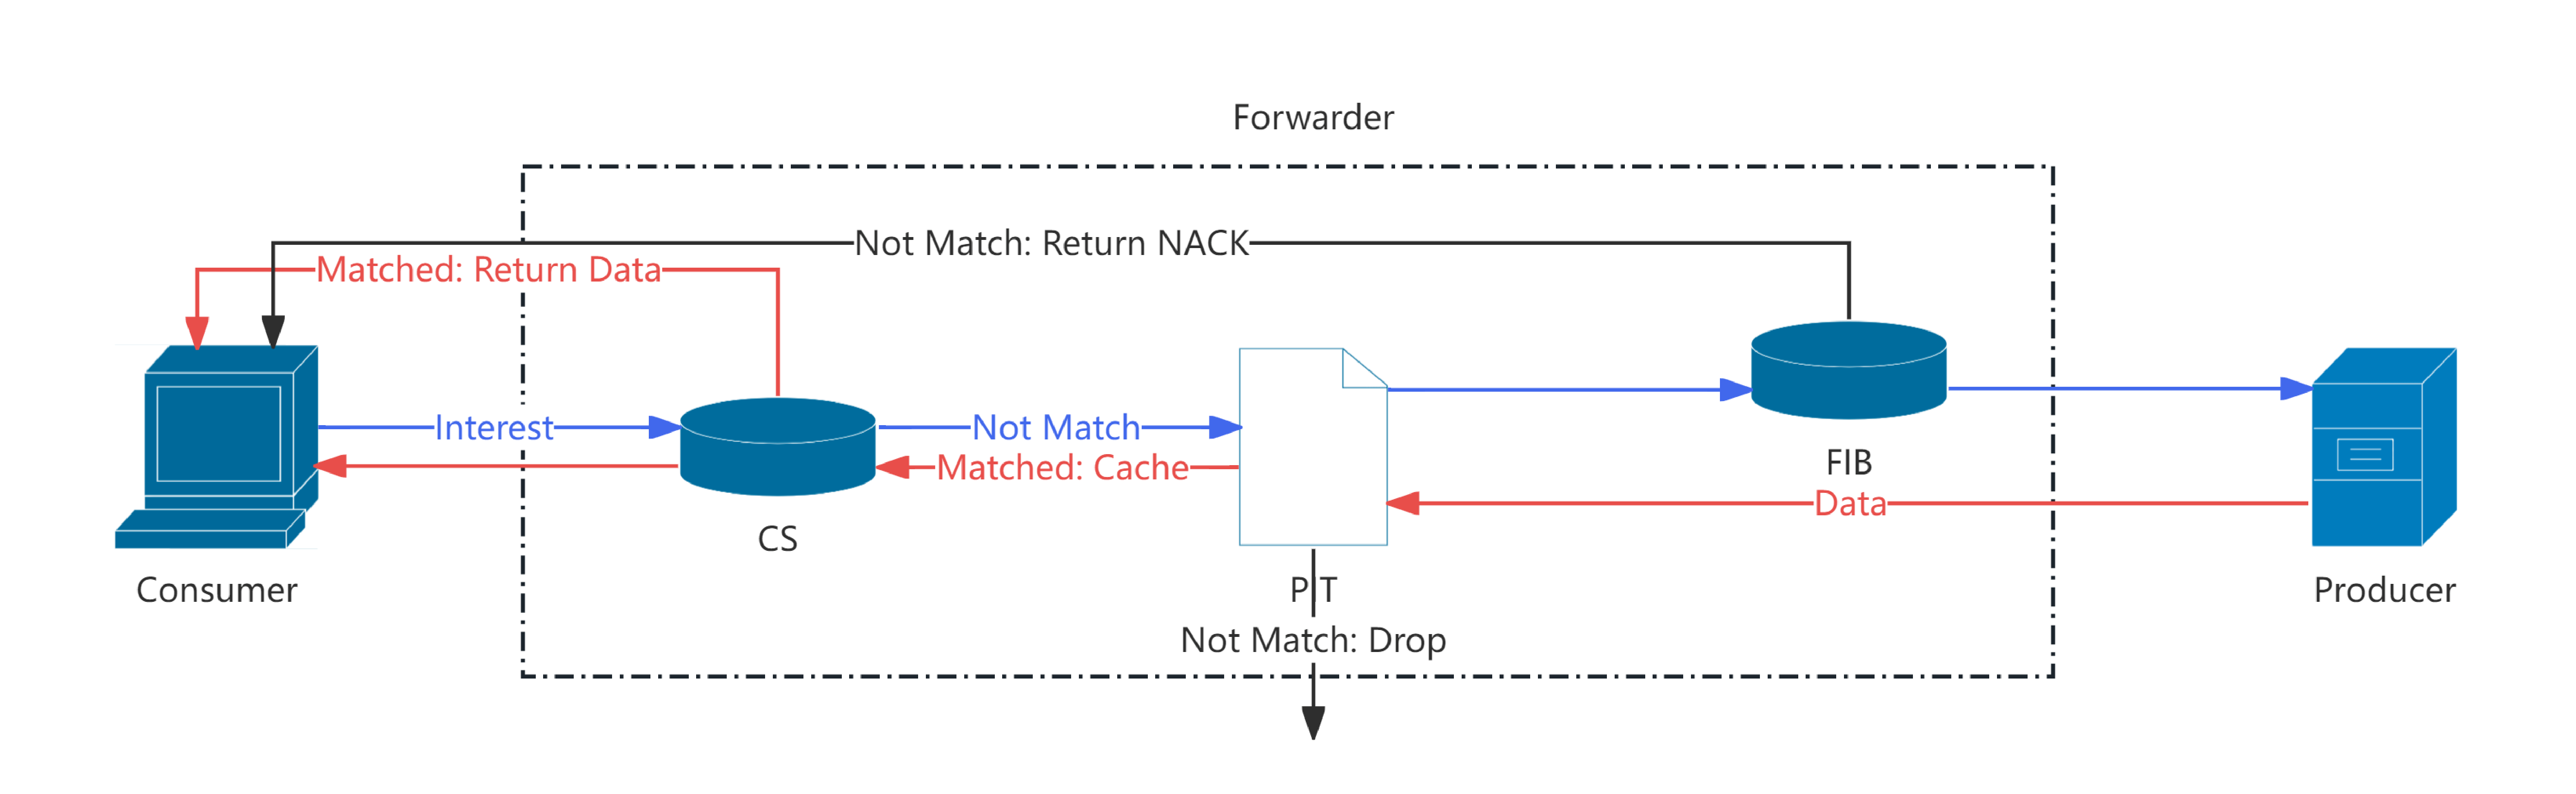
\includegraphics[width=1\linewidth]{NDN Packets Processing Flow.pdf}
    \caption{NDN Packets Processing Flow \csp{Update to make readable in single column form}}
    \label{fig:NDN Packets Processing Flow}
\end{figure}

To maintain and update forwarding paths dynamically, NDN uses the Named-Data Link State Routing protocol (NLSR). This disseminates routing information via Link State Advertisements (LSAs) that carry link status and available data prefix information. Each node periodically exchanges LSAs with its neighbours, builds a comprehensive Link State Database (LSDB), and calculates optimal forwarding paths using link state algorithms like Dijkstra. These calculated paths are stored in each node's FIB, directing Interest Packet forwarding effectively.

Through periodic updates, NLSR quickly adapts to network changes, such as node failures, new node attachments, or topology changes. However, due to its dependence on periodic and network-wide dissemination of routing updates, NLSR can introduce significant latency during rapid producer mobility events, highlighting the necessity for specialised mobility management mechanisms in dynamic scenarios.

\subsection{Producer Mobility Problems}
\csp{This section would benefit from some simulation results to show the extent of the problem.}

Producer mobility in NDN poses significant challenges, especially in dynamic network environments. Each time a producer moves, it needs to re-register its data prefix so that NLSR can propagate the updated routing information across the network. However, routing convergence through NLSR is inherently slow due to periodic dissemination of Link State Advertisements and gradual propagation of routing updates. Until the network fully converges, the interest packets sent by consumers may still follow outdated paths, leading to temporary communication interruptions. Figure~\ref{fig:NDN Producer Mobility Problem} illustrates this problem clearly, showing how routing updates after producer movement cause a disruption in data delivery. \csp{To illustrate the problem, the figure should show the topology with packets being misdirected somehow; the current figure doesn't help.}

\begin{figure}[h]
    \centering
    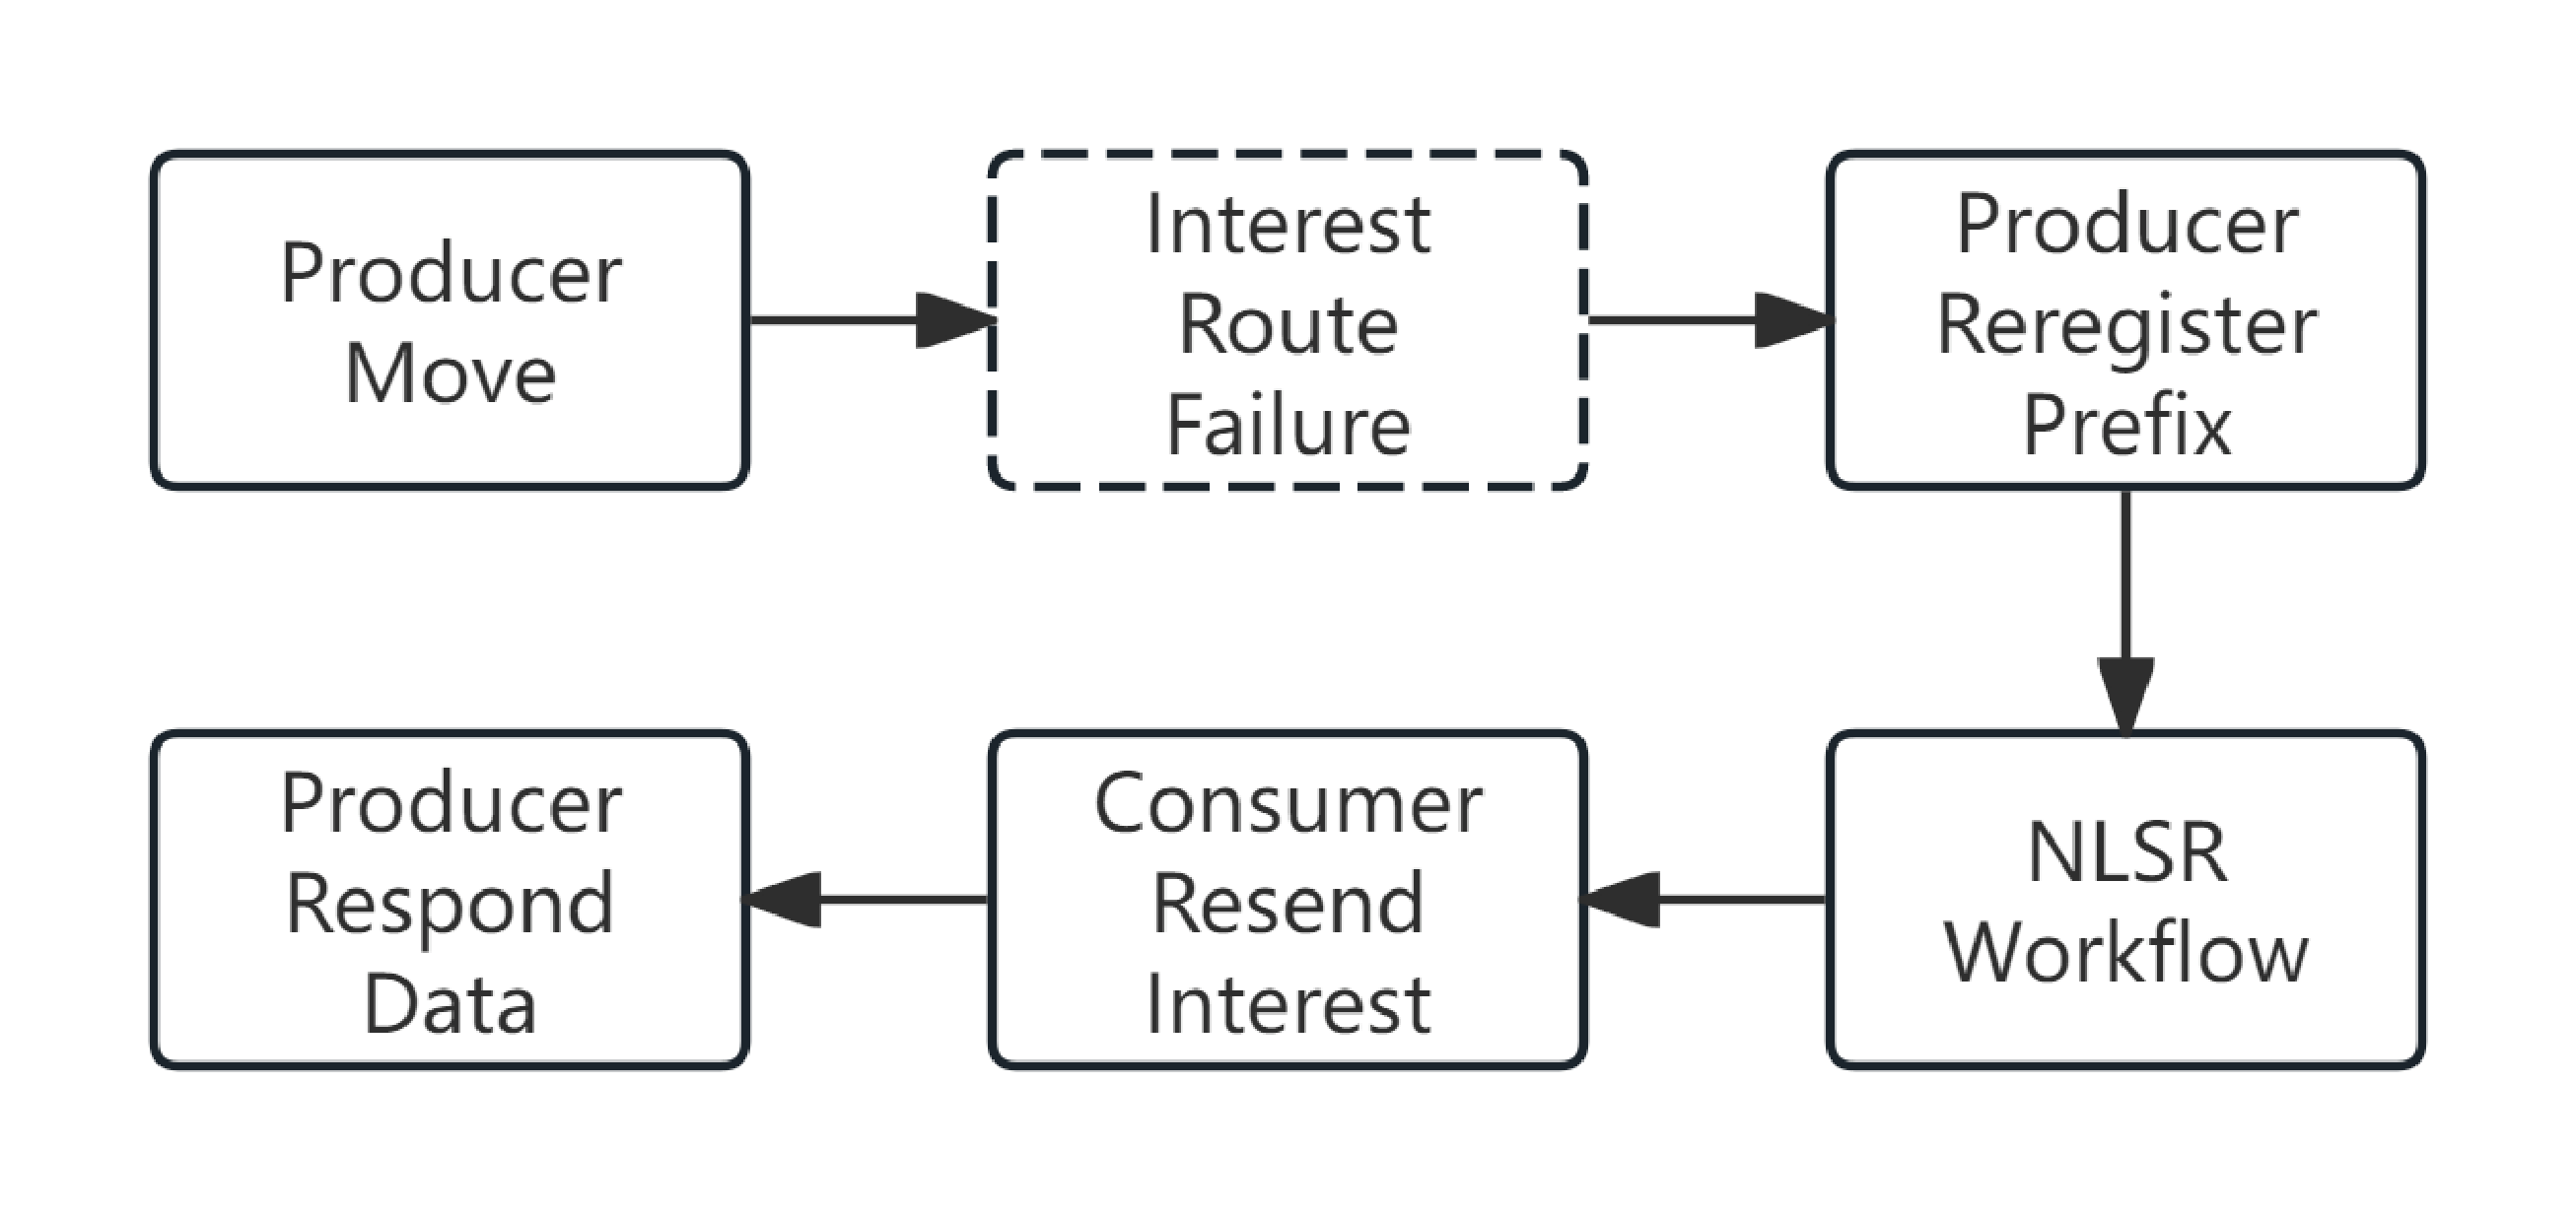
\includegraphics[width=1\linewidth]{NDN Producer Mobility Problem.pdf}
    \caption{NDN Producer Mobility Problem}
    \label{fig:NDN Producer Mobility Problem}
\end{figure}

The specific challenges arising from producer mobility are summarised below.

\textbf{Latency:} When a producer changes its attachment point, the associated data prefix must be re-advertised, initiating routing updates starting from the directly connected forwarder. These updates must propagate throughout the entire network before Interests can reach the producer at its new location. During this routing convergence interval, consumers experience significant communication interruptions, often lasting several seconds or longer. In scenarios requiring low latency, such as live video streaming or real-time conferencing, even brief interruptions degrade the user experience and severely limit NDN's practical deployment.

\textbf{Packet Loss:} During producer relocation and the subsequent routing convergence process, Interest packets arriving at the producer's previous attachment point are unable to reach the new location, causing these packets to expire and be discarded. Additionally, data packets responding to interest received prior to relocation may be stranded at nodes lacking proper PIT entries, as the reverse paths have been invalidated. Without a valid return path, these Data packets remain undeliverable until their lifetimes expire, leading to further packet loss and negatively affecting communication reliability.

\textbf{Increased Network Resource Usage:} The inefficiencies introduced by latency and packet loss also result in increased retransmissions of interest packets. These retransmissions consume additional bandwidth and processing resources across the network, potentially impacting overall network performance and affecting other communications.

These problems highlight the limitations of traditional routing-based approaches, such as NLSR, in handling frequent producer mobility. Addressing these issues effectively requires specialised mechanisms that can rapidly establish temporary communication paths without waiting for global routing convergence.


\section{Controllable Flooding for NDN Mobility} 
\label{sec:solution}

To address the challenges of producer mobility in NDN, particularly in latency-sensitive applications such as video conferencing or live streaming, we propose \textit{OptoFlood}, a comprehensive and controllable flooding mechanism. OptoFlood rapidly establishes temporary bidirectional communication paths immediately following producer movements and leverages these paths to accelerate global routing convergence. Our approach selectively incorporates beneficial elements from existing mobility solutions such as MAP-Me's scoped flooding and KITE's trace-guided forwarding to further improve efficiency and performance.

\csp{Need a diagram showing the operation of the flooding, that the following can refer to.}

\subsection{Producer Mobility Detection and Data Packet Flooding}
\label{sec:solution:data-flooding}

When moving to a new Point of Attachment (PoA), the producer immediately initiates controlled flooding of Data packets corresponding to all Interest packets it had received but had not yet responded prior to handover. These Data packets are marked in their MetaInfo TLV with:
\begin{itemize}
\item \textbf{MobilityFlag}: indicates mobility-related flooding.
\item \textbf{Flood-ID}: unique identifier for deduplication.
\item \textbf{NewFaceSeq}: sequence number that ensures consistency.
\item \textbf{Trace-Hint}: lightweight breadcrumb of recent PoAs (inspired by KITE~\cite{zhang:2018:kite}) for guided flooding.
\end{itemize}

Flooded Data packets preferentially follow existing valid FIB entries. If no valid entry exists, the packets fall back to scoped blind flooding limited by a conservative HopLimit (set to 3), restricting propagation within typical local access and aggregation networks. The goal of this flooding is to reach nodes maintaining valid Pending Interest Table (PIT) entries, thus promptly rescuing pending Interests.

\subsection{Interest Flooding Triggered by Forwarder FIB Invalidation}
\label{sec:solution:interest-flooding}

Forwarders adjacent to the previous PoA detect invalid FIB entries upon receiving Interest packets without available next hops. These forwarders initiate controlled flooding of only the initial batch of Interests directly impacted by producer relocation. Flooding is triggered explicitly after the forwarder observes explicit invalidation signals, such as receiving NACK packets or reaching a predefined consecutive Interest failure threshold.
The Interest flooding strategy involves:
\begin{itemize}
\item \textbf{Prioritised Forward}: Forwarders first attempt to forward Interests via existing valid FIB entries towards known or recent PoAs, guided by \textit{Trace-Hints} embedded within Interest packets.
\item \textbf{Scoped Blind Flooding}: In the absence of valid FIB entries, forwarders employ scoped blind flooding inspired by the local discovery mechanism of MAP-Me~\cite{auge:2016:map-me}, restricting packet propagation by using a conservative HopLimit (typically set to 3).
\end{itemize}

This controlled flooding efficiently discovers the producer's new location, minimizing unnecessary network load.

\subsection{Temporary Bidirectional Path Establishment}
\label{sec:solution:bidir}

OptoFlood leverages the coordinated flooding of Interest and Data packets to establish robust temporary bidirectional paths. When flooded Interests reach the relocated producer, returning Data packets carry updated \textit{NewFaceSeq} and \textit{Flood-ID}. Forwarders receiving these Data packets establish or update a separate Temporary FIB (TFIB), distinct from the standard FIB, specifically designed to handle transient mobility-related paths.
\csp{Why a temporary FIB rather than state in the existing FIB?}

TFIB entries maintain temporary forwarding states with a brief TTL (approximately one second \csp{why this value?}), a duration selected to promptly remove transient forwarding states after global routing convergence, thereby minimizing memory and state overhead.

Flooded Data packets returning downstream primarily follow existing PIT entries towards consumers. If PIT entries have expired, the packets return to TFIB entries, ensuring reliable downstream connectivity.

Thus, the combination of controlled Interest and Data packet flooding rapidly and effectively bridges temporary communication gaps caused by producer mobility, ensuring minimal disruption for latency-sensitive applications.


\subsection{Accelerated Network Convergence}
\label{sec:solution:convergence}

OptoFlood uniquely integrates temporary flooding-based paths with global routing convergence via Named-data Link State Routing (NLSR) \cite{}. Whenever a forwarder establishes a TFIB entry due to successful flooding, it immediately generates and disseminates a short-lived \csp{What is meant by ``short-lived''?} Fast-LSA, which includes the \textit{NewFaceSeq} and face information learned from flooding results. The reason Fast-LSAs are generated only upon TFIB creation, rather than upon other forms of mobility detection, is that TFIB entries explicitly confirm new valid forwarding paths identified by successful flooding. In contrast, other unverified mobility detections could introduce erroneous information or routing instability. This Fast-LSA rapidly propagates among neighboring nodes, typically within milliseconds, significantly accelerating local route convergence. Regular periodic LSAs subsequently replace these Fast-LSAs, allowing TFIB entries to gracefully expire. This approach accelerates global convergence without requiring core NLSR modifications.

\subsection{Security and Flooding Control}

To help mitigate security risks associated with flooding, OptoFlood employs three complementary mechanisms.

First, NDN Data packets contain digital signatures that authenticate static packet fields such as names and content, protecting packet integrity and authenticity from intermediate node manipulation. %Dynamic fields like \textit{MobilityFlag} (changed upon PIT match) and \textit{HopLimit} (decremented hop-by-hop) cannot be authenticated via signatures, as a legitimate intermediate modification occurs. Thus, signatures provide baseline authenticity rather than complete tamper protection for dynamic fields.

Second, a global maximum HopLimit threshold (\S\ref{sec:solution:data-flooding}) is enforced network-wide, derived from typical mobile network hop distances between PoAs. This prevents malicious producers from initiating flood attacks with excessive hop counts, ensuring that flooding remains confined to local access or aggregation layers.

Third, strict flood rate limits per-producer (60–100 packets/second) prevent resource exhaustion, effectively protecting against Denial-of-Service (DoS) attacks by restricting flood volumes within realistic network capacity limits.

Together, these mechanisms maintain a robust security posture without significantly increasing complexity or overhead.

\section{Experiment}
\subsection{Experimental Design}
This experiment evaluates and compares the performance of traditional NDN global routing mechanisms with our proposed OptoFlood approach in the context of producer mobility. We specifically simulate real-time video transmission scenarios to assess key metrics, including latency, packet loss rate, and network overhead, under dynamically changing network conditions.

We chose video streaming as our primary test scenario due to its high sensitivity to latency and packet loss, making it ideal for clearly highlighting performance differences. In addition, scenarios such as mobile video conferencing and live streaming from moving vehicles are common, underscoring the practical importance of efficiently managing producer mobility.

\subsubsection{Consumer Application}

The consumer application continuously issues Interest packets and processes received Data packets to simulate realistic, real-time video stream handling. Maintains a straightforward NDN-based operation without explicit mobility awareness, relying instead on the underlying network mechanisms provided by OptoFlood.

\textbf{Automatic Data Requests:}
The consumer sends Interests with a predefined name prefix (e.g., \texttt{/example/livestream/}) appended by sequential version numbers to uniquely identify each data chunk. The interest packets are marked as "must be fresh" and set with a lifetime of 6 seconds to ensure timely delivery, aligning with typical real-time video requirements (simulating 30 frames per second).

\textbf{Request Frequency:}
The application generates Interest packets at intervals of 33 milliseconds, simulating the typical frame rate of a real-time video stream. This frequency ensures realistic load conditions without overwhelming network resources.

\textbf{Management of Unresponsive Interests:}
Timed-out Interests are placed into a First-In-First-Out (FIFO) queue for retransmission at a controlled, lower frequency of once per second. Retransmissions are triggered by Interest timeouts or Negative Acknowledgments (NACKs), such as "NoRoute" or "NotFound", indicating possible mobility-related disruptions. This conservative retransmission policy minimises resource consumption while maintaining stream continuity.

\textbf{Data Reception and Verification:}
Upon receiving Data packets, the consumer verifies their authenticity using a preloaded trust schema—a predefined set of rules for packet signature verification—to ensure data integrity and security. Verified Data packets simulate video frame processing by logging content reception; verification failures trigger error logging.

\textbf{Error Handling:}
Received NACK packets result in logging the error cause and scheduling the Interest for controlled retransmission. Similarly, timeouts prompt retransmission without requiring explicit mobility management at the application layer, as forwarders transparently handle temporary flooding and recovery paths.

\textbf{Naming and Integrity:}
Strict naming conventions are maintained to ensure accurate matching of requested and received Data packets, preserving stream integrity.

In general, the consumer remains lightweight, relying on standard NDN operations and OptoFlood’s underlying flood mechanisms to manage mobility transparently.

\subsubsection{Producer Application}

The producer application generates Data packets in response to Interests and incorporates necessary mobility indications to enable OptoFlood’s controlled flooding and route convergence acceleration. The application itself remains primarily focused on standard data processing tasks, with mobility handled through simple packet markings.

\textbf{Prefix Registration:}
The producer advertises its data prefix (e.g., \texttt{/example/testApp}) to the network using standard NLSR commands (e.g., \texttt{nlsrc advertise}), enabling correct Interest forwarding.

\textbf{Interest Packet Processing:}
Upon receiving an Interest packet matching its prefix, the producer promptly generates and returns the corresponding Data packet, setting a freshness period of 10 seconds to ensure timeliness aligned with typical video application requirements.

\textbf{Data Content Generation and Signing:}
Data payloads in the current experiment use placeholder strings (e.g. "Hello, world!") to simulate real-time data characteristics. Although not employing actual video content, these payloads maintain consistent sizes to reflect realistic video packet profiles. Generated Data packets are digitally signed using the default keychain, ensuring integrity and security.

\textbf{Mobility Detection and Flooding Preparation:}
Upon detecting changes in network attachment (such as switching to a new Point of Attachment), the producer marks pending Data packets with a \texttt{MobilityFlag} within the MetaInfo TLV.of the packet. Additionally, each marked packet includes a unique Flood-ID (for duplicate detection), a sequence number (ensuring correct ordering and consistency), and a trace-hint (a lightweight path indicator derived from recent attachment points, guiding packet direction during flooding). These markings prepare Data packets for controlled flooding, rescuing pending Interests affected by mobility events.

\textbf{Controlled Data Packet Flooding:}
Marked Data packets are flooded starting from the new PoA. Flooding prioritizes forwarding based on existing FIB entries whenever possible, resorting to limited, scoped flooding (1–2 hops) only when no valid FIB entries exist. Controlled flooding employs hop-limit restrictions and trace-hints to ensure efficient propagation toward nodes on the previous forwarding paths.

\textbf{Error Handling:}
Prefix registration failures result in error messages and termination of forwarding operations to prevent unnecessary resource usage. Mobility events and packet marking actions are logged internally but do not disrupt application operation, as forwarders handle the flooding process transparently.

This design ensures real-time responsiveness, relying on OptoFlood to manage producer mobility without placing undue complexity on the application itself.

\subsubsection{Network Topology}
The experiment was constructed using a classic three-layer mobile network model, including:
\begin{itemize}
    \item Core layer: 1 core layer switch.
    \item Distribution layer: 2 aggregation layer switches, each connected to the core layer switch.
    \item Access layer: Each aggregation layer switch is connected to 3 access layer switches.
    \item Core-to-distribution connection: 1 Gbps bandwidth, 1 ms latency.
    \item Distribution-to-access connection: 1 Gbps bandwidth, 1 ms latency.
    \item Access-to-client connection: 100 Mbps bandwidth, 10 ms latency.
\end{itemize}

\begin{figure}
    \centering
    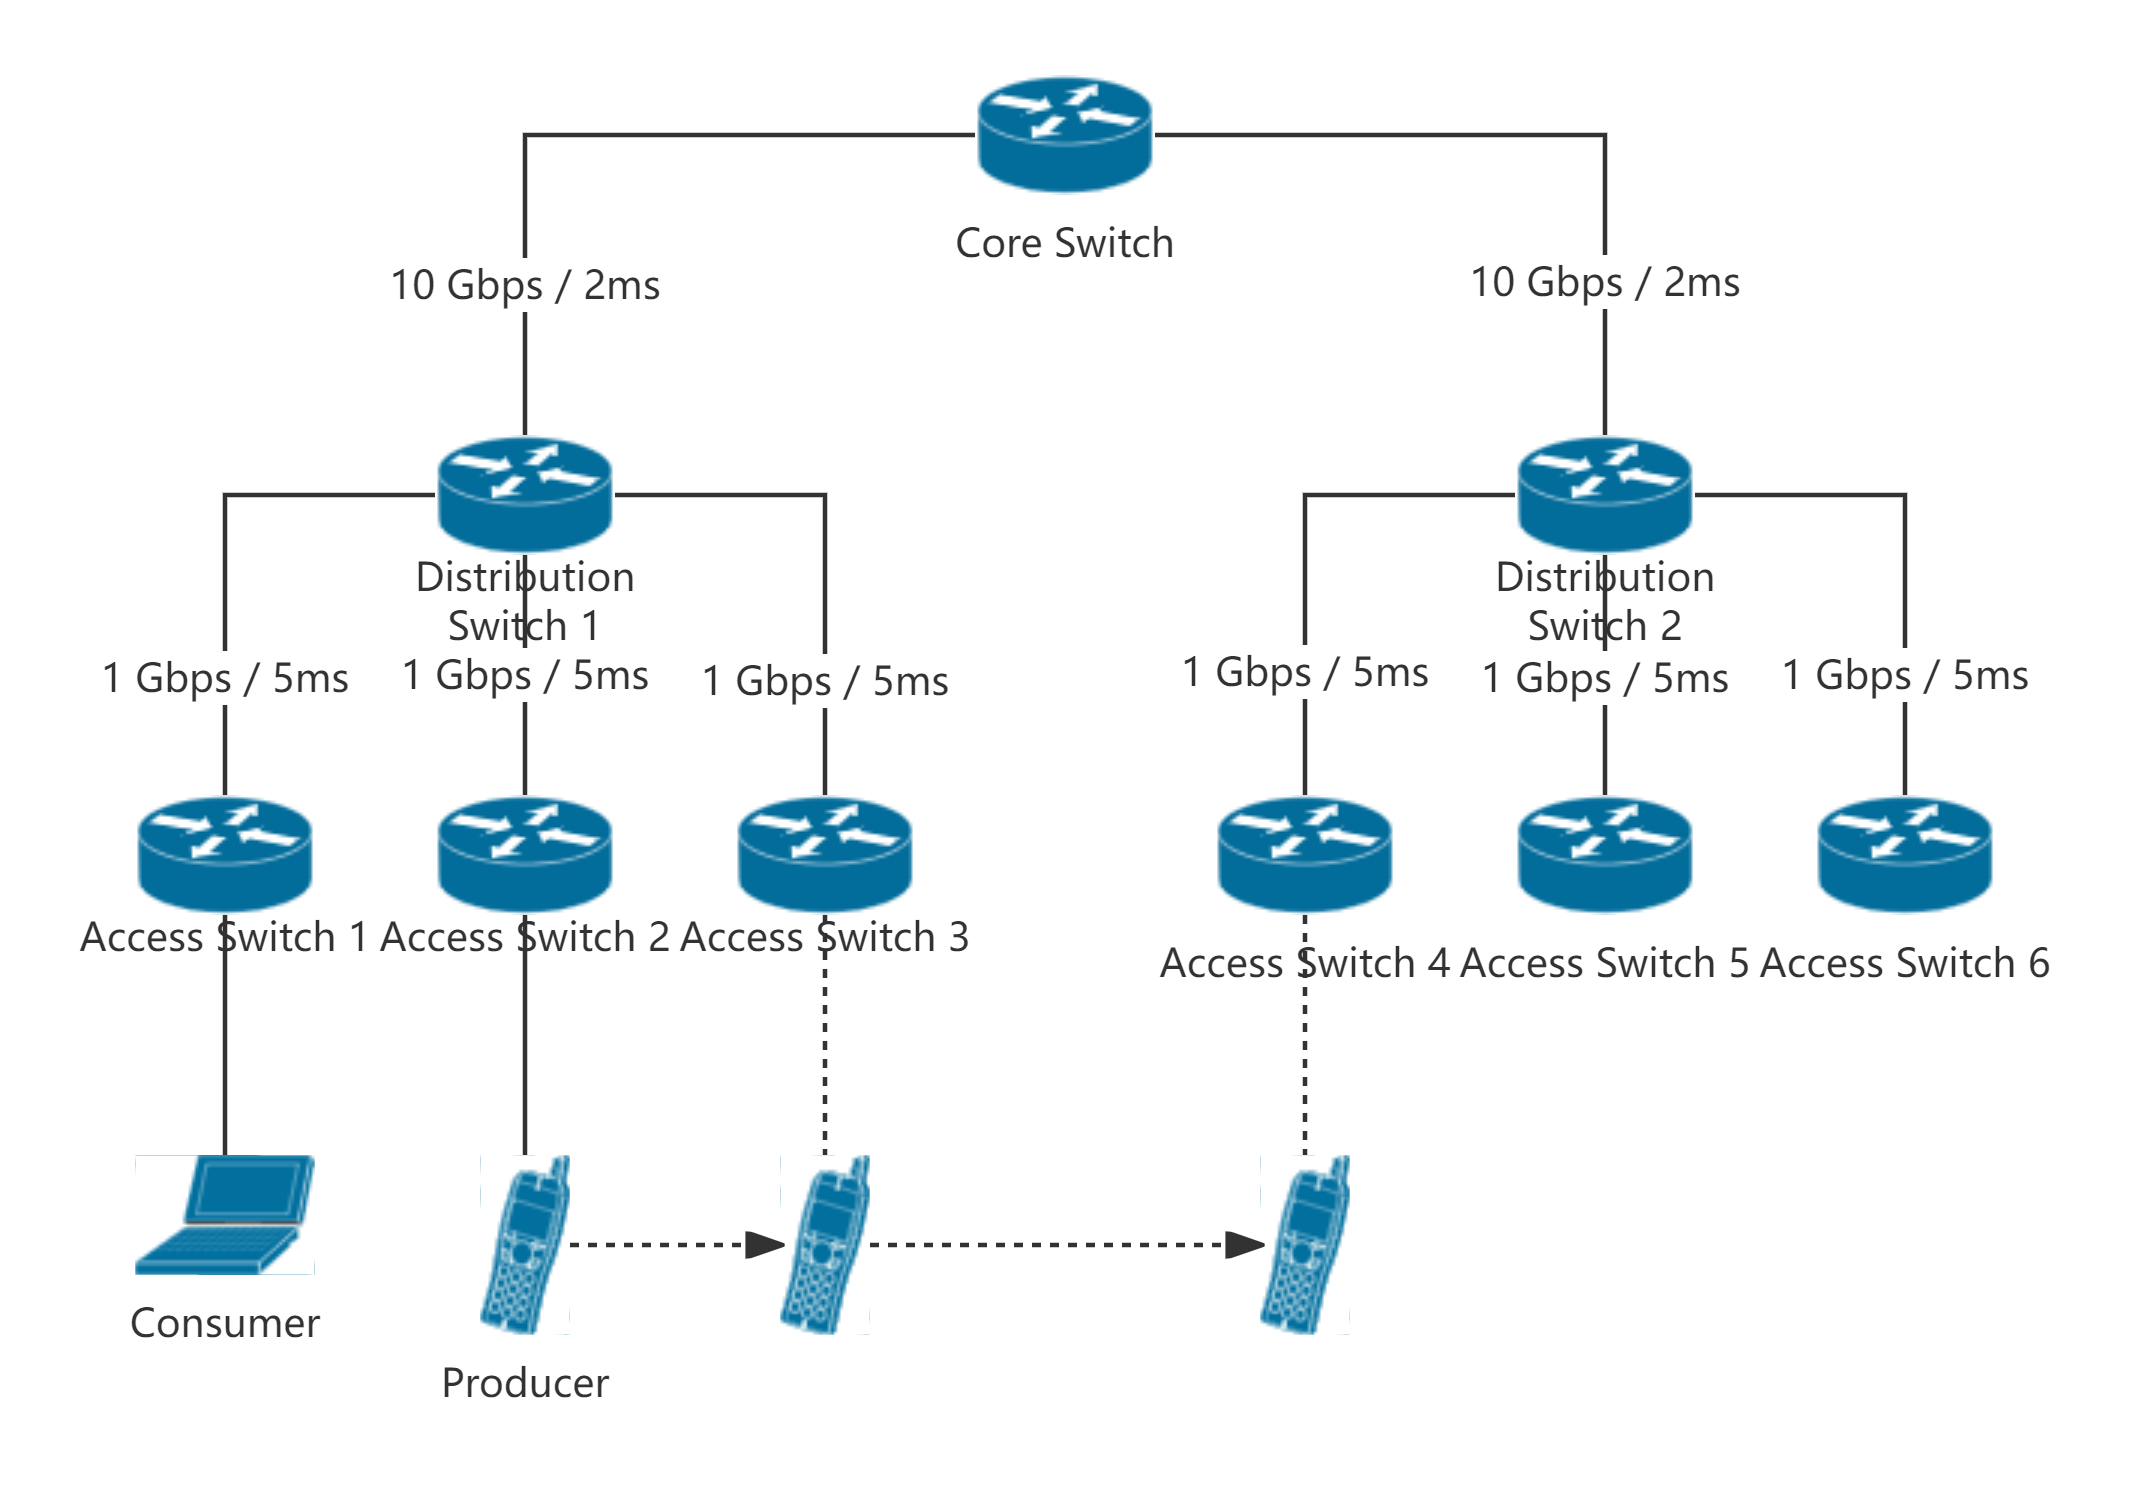
\includegraphics[width=\columnwidth]{Topology.png}
    \caption{Experiment}
    \label{fig:enter-label}
\end{figure}

\subsection{Baseline Test}
This experiment aims to evaluate the impact of producer mobility in NDN on video transmission performance, especially when the new mechanism (controlled flooding) is not enabled. The experiment measures the impact of producer mobility in the network topology on latency, packet loss rate, and network response time. The experiment is conducted in the Mini-NDN simulation environment, with consumer and producer applications running on designated nodes respectively.

\csp{Unnecessary detail: the next three paragraphs can be compressed to one or two sentences}

First, start the Mini-NDN environment and initialize all network nodes. During the startup process, NFD and NLSR are started on all nodes. In this step, wait for the NLSR protocol to start and reach a stable state, which can usually be achieved within 20 seconds to ensure that the network routing information is correctly propagated and stable.

After the network configuration is completed, start the tcpdump tool on the consumer node to listen and capture packets in the network and save them as consumer\_capture.pcap file for subsequent analysis. This step provides a detailed record of network communication during the experiment, which can help accurately analyze the impact of producer mobility on network performance.

Next, start the producer application on the producer node and the consumer application on the consumer node at the same time. The producer application is responsible for processing the interest packet request sent by the consumer and returning the corresponding data packet, while the consumer application periodically sends interest packets to request data. This process simulates the common data request and transmission behavior in real-time video streaming applications.

The core part of the experiment is to simulate the movement of the producer in the network. First, the producer is connected to the initial access switch (acc2). After a period of stable operation (30 seconds), the producer is moved from the initial access switch (acc2) to another access switch (acc3). This operation is achieved by disconnecting the producer from the current access switch and establishing a connection with the new access switch. After another 30 seconds of stable operation, the producer is moved again to another new access switch (acc4) to simulate multiple movements of the producer between different layers in the network. These movement operations are used to observe and measure the impact of producer movement on data transmission performance, including changes in transmission delay and packet loss rate.
\csp{Why 30 seconds? Not clear what type of system is being simulated}

After the experiment, stop data capture and terminate the tcpdump process, and then analyze the captured data file consumer\_capture.pcap to evaluate the specific impact of producer mobility on network performance. Finally, the operation status of the network can also be checked and verified through the command line interface of Mini-NDN to ensure the accuracy and reliability of the experimental results.
\csp{Unnecessary detail}

This experiment systematically simulates the movement of producers in the network and provides benchmark data for evaluating producer mobility issues in the NDN environment. These data will provide an important reference for subsequent research on the application effect of optimization mechanisms in producer mobility scenarios.
\csp{Lacks depth: what type of producer moving in what envirnment?}

\begin{figure}
    \centering
    \includegraphics[width=\columnwidth]{baseline_throughput.jpg}
    \caption{baseline}
    \label{fig:enter-label}
\end{figure}

\subsection{Solution Test}

\begin{figure}
    \centering
    \includegraphics[width=\columnwidth]{solution_throughput.jpg}
    \caption{solution}
    \label{fig:enter-label}
\end{figure}

\subsection{Data Collection}
\csp{Why are these the right metrics?}
\begin{itemize}
    \item Intra-segment latency: Measures the time from when the producer sends each video segment to when the consumer receives it. This will help understand the impact of producer movement on individual packet transmission efficiency.
    \item Movement delay: Pay special attention to the additional delay caused when the producer's location changes. This can be evaluated by comparing the transmission latency of the same video clip before and after the producer moves between different access layer switches.
    \item Overall network response time: When the producer changes location and starts sending video data to when the consumer first receives the changed data. This metric captures how quickly the network responds to changes in producer location.
    \item Packet loss rate: The ratio of requested packets to successfully received packets.
    \item Network usage: The total bandwidth usage of the network during the experiment.
\end{itemize}

\section{Analysis}
This section will analyze in detail the performance of the controlled flooding mechanism in a dynamic network scenario. The analysis will be based on a simulated network environment, focusing on evaluating the improvement effect of the flooding mechanism on the producer mobility problem, including key performance indicators such as network latency, packet loss rate, and network resource utilization.

\subsection{Theoretical Analysis of Network Performance}
Delay reduction: It is expected that the delay of data transmission will be reduced by adopting the controlled flooding mechanism. Since packets can be propagated immediately without waiting for global routing updates, the data transmission time after the producer's location changes should be faster than the traditional global routing update mechanism.

Packet loss rate: In a dynamic network environment, especially in scenarios where producers move frequently, traditional routing update methods may result in high packet loss rates. The controlled flooding mechanism reduces such problems by quickly responding to location changes, thereby improving the reliability of data transmission.

Network load management: Although the flooding mechanism may increase the initial network load, the occupation of network resources can be effectively controlled through appropriate control strategies, such as hop limit and packet life cycle management, thereby optimizing the overall network performance.

\csp{Why are the above the right metrics?}

\subsection{Discussion of expected results}
Based on the above theoretical analysis, we can predict that the controlled flooding mechanism performs well in reducing latency and improving data transmission reliability. In addition, although the network resource utilization may increase in the early stage of the experiment, in the long run, the overall resource efficiency of the network should be improved.

\section{Related Work}

The management of producer mobility in NDN has attracted significant research attention. Various solutions have emerged, generally categorised according to their underlying mechanisms. Here, we summarise three representative approaches—KITE, AFIRM, and MAP-Me—and highlight their respective strengths and limitations.

\textbf{KITE} \cite{KITE} employs an anchor-based approach by establishing explicit tracking paths between a mobile producer and a stationary anchor node. The producer periodically issues authenticated trace Interests towards the anchor, creating a breadcrumb-like trail to its latest location, thus facilitating hop-by-hop routing. KITE is straightforward and robust, significantly reducing dependency on global routing updates by continuously maintaining explicit anchor-based paths. However, its reliance on anchor nodes inherently introduces potential bottlenecks and single point of failure, especially in scenarios involving intense or large-scale producer mobility.

\textbf{AFIRM (Adaptive Forwarding-based Link Recovery for Mobility)} \cite{AFIRM} addresses producer mobility through adaptive repair of forwarding paths, without relying on an anchor node. Upon detecting producer mobility, AFIRM proactively sends special "recovery" packets carrying mobility indicators along both old and new forwarding paths, quickly updating Forwarding Information Base (FIB) entries at intermediate nodes. These rapid and localised updates effectively minimise disruptions, making AFIRM particularly suitable for scenarios involving frequent and localised movements. However, AFIRM's performance strongly depends on the timely and accurate detection of mobility events. In highly dynamic environments, the frequent generation and propagation of recovery packets may lead to increased signalling overhead.

\textbf{MAP-Me (Managing Anchor-less Producer Mobility)} \cite{MAPME} similarly provides anchor-less mobility support, entirely handling producer location updates within the data plane via special Interest packets. Whenever the producer moves, MAP-Me generates immediate Interest notifications that proactively propagate new location information to affected forwarding paths, avoiding the delays associated with global routing updates or anchor nodes. MAP-Me thus excels in latency-sensitive contexts such as live video streaming due to its responsiveness and low handoff delays. However, under conditions of frequent and high-intensity mobility, MAP-Me's aggressive local updates may generate considerable overhead, potentially impacting network resource usage.

In terms of route updates, KITE periodically disseminates authenticated trace Interests towards the anchor node, thereby maintaining a continuous breadcrumb trail. In contrast, AFIRM sends explicit "recovery" packets immediately upon detecting producer mobility events, ensuring rapid local path updates. MAP-Me proactively generates Interest notifications upon every movement, swiftly propagating new forwarding states throughout affected network segments. All three differ fundamentally from the baseline NDN, where routing updates rely primarily on periodic global advertisements, resulting in slow convergence and increased disruptions during mobility.

In comparison, our OptoFlood solution offers a comprehensive flooding-based mechanism specifically designed for dynamic producer mobility scenarios, employing controlled flooding of both Data and Interest packets immediately following producer movement. Unlike KITE, OptoFlood does not depend on anchor nodes, avoiding potential single points of failure and path inefficiencies. Compared to AFIRM and MAP-Me, which rely heavily on explicit route-update packets, OptoFlood leverages a proactive flooding strategy to rescue pending Interests instantly, significantly reducing latency and retransmission overhead. Moreover, by integrating temporary flooding-based paths with Named-data Link State Routing (NLSR), OptoFlood generates short-lived local LSAs, accelerating global routing convergence compared to traditional periodic routing updates.

\csp{add discussion of Cullen Jennings' MoQ work, which has a very NDN flavour}

\section{Conclusion and Future Work}
\subsection{Conclusion}
WORKING IN PROGRESS...
\subsection{Long Term Impact Assessment}
\subsubsection{Continuous optimization of network performance}
\begin{itemize}
    \item Efficiency Improvements: Long-term application of this strategy may lead to continued improvements in the network's overall efficiency, especially in data transfer speeds and reduced latency.
    \item Enhanced Reliability: The network may gradually adapt to new propagation mechanisms over time, improving overall data transmission reliability.
\end{itemize}

\subsubsection{Resource Usage and Network Stability}
\begin{itemize}
    \item Resource Optimization: Long-term implementation may lead to more efficient use of network resources, especially regarding packet propagation and drop strategies.
    \item Stability Analysis: Evaluate the impact of this strategy on network stability over time, especially in the face of high loads and dynamic changes.
\end{itemize}

\subsection{Future Development Direction}
Discuss how this strategy can be further optimized to adapt to changes in the future network environment as technology develops. Consider possible future application scenarios of this strategy, such as the Internet of Things, smart cities, etc.


\section*{Acknowledgment}

The preferred spelling of the word ``acknowledgment'' in America is without 
an ``e'' after the ``g''. Avoid the stilted expression ``one of us (R. B. 
G.) thanks $\ldots$''. Instead, try ``R. B. G. thanks$\ldots$''. Put sponsor 
acknowledgments in the unnumbered footnote on the first page.

\section*{References}

Please number citations consecutively within brackets \cite{b1}. The 
sentence punctuation follows the bracket \cite{b2}. Refer simply to the reference 
number, as in \cite{b3}---do not use ``Ref. \cite{b3}'' or ``reference \cite{b3}'' except at 
the beginning of a sentence: ``Reference \cite{b3} was the first $\ldots$''

Number footnotes separately in superscripts. Place the actual footnote at 
the bottom of the column in which it was cited. Do not put footnotes in the 
abstract or reference list. Use letters for table footnotes.

Unless there are six authors or more give all authors' names; do not use 
``et al.''. Papers that have not been published, even if they have been 
submitted for publication, should be cited as ``unpublished'' \cite{b4}. Papers 
that have been accepted for publication should be cited as ``in press'' \cite{b5}. 
Capitalize only the first word in a paper title, except for proper nouns and 
element symbols.

For papers published in translation journals, please give the English 
citation first, followed by the original foreign-language citation \cite{b6}.

\bibliographystyle{IEEEtran}
\bibliography{conference_101719}
\end{document}
